\hypertarget{table-of-contents}{%
\section{Table of contents}\label{table-of-contents}}

\begin{enumerate}
\def\labelenumi{\arabic{enumi}.}
\tightlist
\item
  Abstract
\item
  Introduction

  \begin{enumerate}
  \def\labelenumii{\arabic{enumii}.}
  \tightlist
  \item
    Purpose of research
  \item
    Tools and methodology

    \begin{itemize}
    \tightlist
    \item
      The Rapsberry Pi (RPi)
    \item
      Ansible
    \item
      The study of Enzyme kinetics
    \end{itemize}
  \end{enumerate}
\item
  Project process

  \begin{enumerate}
  \def\labelenumii{\arabic{enumii}.}
  \tightlist
  \item
    RPi preparation

    \begin{itemize}
    \tightlist
    \item
      OS installation
    \item
      SSH and/or VNC
    \end{itemize}
  \item
    RStudio and Shiny Server

    \begin{itemize}
    \tightlist
    \item
      Installation
    \item
      General information
    \end{itemize}
  \item
    PMM - Pi Michaelis Menten

    \begin{itemize}
    \tightlist
    \item
      Development
    \item
      Deployment
    \end{itemize}
  \item
    Security measures
  \end{enumerate}
\item
  Possible problems and their solutions
\item
  Results
\item
  Discussion
\item
  Conclusion
\end{enumerate}

\newpage

\hypertarget{abstract}{%
\section{Abstract}\label{abstract}}

In this dissertation, I examine whether (1) if it's possible to use the
Raspberry Pi, a palm-sized computer, as the host for a web application
(WebApp), developed in the RStudio IDE, that can compute complex
mathematical formulas in real-time, in our case: the well-known
Michaelis-Menten model, which is widely used in the study of enzyme
kinetics; and (2) with the help of the Shiny framework to develop a
user-friendly interface and host the WebApp, henceforth called Pi
Michaelis-Menten or PMM for short, on a local area network (LAN) or
futhermore, to deploy it to the internet (WAN).

\hypertarget{introduction}{%
\section{Introduction}\label{introduction}}

\hypertarget{purpose-of-research}{%
\subsection{Purpose of research}\label{purpose-of-research}}

The world is advancing rapidly into the digital space, making it's a
necessary to develop futher our servers and databases for world wide
uses. Thereby, I suggest that the RPi will be able to perform these two
tasks exceptionally well, and is an affordable, easy-to-use solution for
web hosting and sharing projects, especially for personal uses.

To demonstrate its capabilities, I chose to build a web application
written in R language, that utilizes the Michaelis-Menten model,
calculating the speed of an enzyme reaction with different parameters.
The results will then be presented in graph-base, thus making it easier
for us to interpret.

To summarize, the research has two main goals, which are: - firstly, if
the Raspberry Pi is sufficient for real-time computation of complex
mathematical formulas, in our case the Michaelis-Menten model. -
secondly, to build a user-friendly interface that allows modification of
input data for the Michaelis-Menten model. The model's results will then
be presented in the form of graphs for easier interpretation.

\hypertarget{tools-and-methodology}{%
\subsection{Tools and methodology}\label{tools-and-methodology}}

\hypertarget{the-raspberry-pi-rpi}{%
\subsubsection{The Raspberry Pi (RPi)}\label{the-raspberry-pi-rpi}}

\hypertarget{brief-history}{%
\paragraph{Brief history}\label{brief-history}}

The palm-sized computere known as the Raspberry Pi is an invention of
four professors at Cambridge University in England. Those four
professors were: Eben Upton, Rob Mullins, Jack Lang and Alan Mycroft.
The idea came to be when the Professors noticed a decrease in skill and
number of A-level students who wanted to study Computer Science /
Informatics. Then they discovered that this was because home computers
had become more and more expensive, which made parents not allowing
their children to experiment with them. So the Professors wanted to look
for an affordable solution that would allow the younger generation to
experiment with computers at home. By 2011, the first model of the
Raspberry Pi was available to the public, with more than 2 million units
sold in the first two years.

\pagebreak

\hypertarget{about-my-4b-model}{%
\paragraph{About my 4B model}\label{about-my-4b-model}}

\begin{itemize}
\tightlist
\item
  Overall specifications:

  \begin{itemize}
  \tightlist
  \item
    CPU: Broadcom BCM2711, Quad core Cortex-A72 (ARM v8) 64-bit SoC @
    1.5GHz
  \item
    PSU: 5V DC via USB-C connector, adapter:
  \item
    RAM: 4GB of LPDDR4-3200 SDRAM
  \item
    ROM: micro-SD card slot
  \item
    Network:

    \begin{itemize}
    \tightlist
    \item
      2.4 GHz and 5.0 GHz IEEE 802.11ac wireless
    \item
      Bluetooth 5.0, BLE
    \item
      Gigabit Ethernet
    \end{itemize}
  \item
    Ports: 2-2 USB 3.0 and 2.0 ports; 2 micro-HDMI; etc.
  \item
    GPIO pins
  \item
    OS: Raspberry Pi OS (buster), previously known as Raspbian
  \end{itemize}
\item
  Things that are crucial to the project:

  \begin{itemize}
  \tightlist
  \item
    consistent internet connection, especially so if running with
    ``Headless'' mode (using the RPi without any peripherals like mouse
    or monitor)
  \end{itemize}
\item
  Things that are recommended to have:

  \begin{itemize}
  \tightlist
  \item
    at least 4GB of RAM
  \item
    cooling fan
  \end{itemize}
\end{itemize}

\textbf{I mostly control my RPi through SSH/terminal so this
dissertation focuses mainly on the command-line when it comes to
installing, editing files etc. For GUI instruction, it's highely advised
to read over the cited documentation sources}

\pagebreak

\hypertarget{enzyme-kinetics}{%
\subsubsection{Enzyme Kinetics}\label{enzyme-kinetics}}

\hypertarget{brief-introduction}{%
\paragraph{Brief introduction}\label{brief-introduction}}

Enzyme kinetics is the study of the rates of enzyme-catalysed chemical
reactions, the reaction rate is measured and the effects of varying the
conditions of the reaction are investigated. Studying an enzyme's
kinetics in this way can reveal the catalytic mechanism of this enzyme,
its role in the metobolism, how its activity is controlled, and how a
drug or a modier might affect the rate.

An enzyme (E) is typically a protein molecule that promotes a reaction
of another molecule, its substrate (S). This binds to the active site of
the enzyme to produce an enzyme-substrate complex ES, and is transformed
into an enzyme-product complex EP and from there to product P, via a
transition state ES*. The series of steps is known as the mechanism:

\begin{quote}
E + S -\textgreater{} ES -\textgreater{} ES* -\textgreater{} EP
-\textgreater{} E + P
\end{quote}

\begin{figure}
\centering
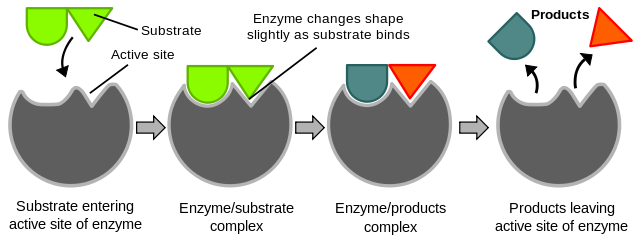
\includegraphics{./media/enzyme_action.png}
\caption{Enzyme reaction}
\end{figure}

\hypertarget{single-substrate-reactions-and-the-michaelis-menten-model}{%
\paragraph{Single-substrate reactions and the Michaelis-Menten
model}\label{single-substrate-reactions-and-the-michaelis-menten-model}}

Enzymes with single-substrate mechanisms include isomerases such as
\emph{triosephosphateisomerase} or \emph{bisphosphoglycerate mutase},
intramolecular lyases such as \emph{adenylate cyclase} and the
\emph{hammerhead ribozyme}, an RNA lyase. Biochemical reactions
invovling a single-substrate enzyme are often assumed to follow
Michaelis-Menten kinetics, regardless of the underlying assumptions of
the model.

In biochemistry, Michaelis-Menten kinetics is one of the best-known
modles of enzyme kinetics. It is named after German biochemist
\emph{Leonor Michaelis} and Canadian physician \emph{Maud Menten}. The
model takes the form of an equation describing the rate of enzymatic
reations, by relating reaction rate \emph{v} (rate of formation of
product \emph{{[}P{]}}) to \emph{{[}S{]}}, the concentration of a
substrate \emph{S}. Its formula is given by:

\begin{quote}
v = d{[}P{]}/dt = Vmax * {[}S{]}/(KM + {[}S{]})
\end{quote}

The above equation is called \textbf{Michaelis-Menten equation}. Here,
\emph{Vmax} represents the maximum rate achieved by the system,
happening at saturating substrate concentration for a given enzyme
concentration. When the value of the Michaelis constant \emph{KM} is
numerically equal to the substrate concentration, then the reaction rate
is half of \emph{Vmax}.

\newpage

\hypertarget{project-process}{%
\section{Project process}\label{project-process}}

\hypertarget{rpi-preparation}{%
\subsection{RPi preparation}\label{rpi-preparation}}

The official documentation is well-written and will help you with almost
any FAQ: \href{https://www.raspberrypi.com/documentation/}{Raspberry Pi
Documentation}. My steps below are mostly identical, and is just a
paraphrase of mine from the documentation.

! It's a good practice to run
\texttt{sudo\ apt\ update\ \&\ sudo\ apt\ upgrade} once in awhile, and
before installing a new package.

\hypertarget{os-installation}{%
\subsubsection{OS installation}\label{os-installation}}

Download the \href{https://www.raspberrypi.com/software/}{Raspberry Pi
Imager}

Before flashing the OS image to the SD card, considering if you need to
use \emph{Headless mode} - controlling the RPi without mouse or monitor.

\hypertarget{headless-ssh-andor-vnc}{%
\subsubsection{Headless: SSH and/or VNC}\label{headless-ssh-andor-vnc}}

\hypertarget{getting-your-rpis-private-ip}{%
\paragraph{Getting your RPi's private
IP}\label{getting-your-rpis-private-ip}}

To find your RPi's private IP address, either login to your router's
dashboard and check the DHCP tab or by using \emph{nmap} -
\href{https://manpages.ubuntu.com/manpages/bionic/en/man1/nmap.1.html}{network
exploration tool}:

\begin{Shaded}
\begin{Highlighting}[]
\ExtensionTok{$}\NormalTok{ nmap }\AttributeTok{{-}A} \OperatorTok{\textless{}}\NormalTok{your\_subnet\_IP}\OperatorTok{\textgreater{}}\NormalTok{/24}
\end{Highlighting}
\end{Shaded}

The -A flag/option will output a lot of extra information, you need to
look for the following lines

\begin{figure}
\centering
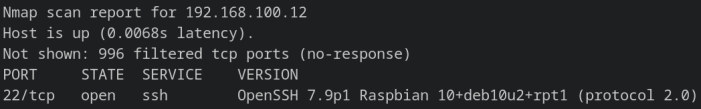
\includegraphics{./media/RPi_ip.png}
\caption{RPi private IP}
\end{figure}

Another cli tool is \emph{ping} which is simpler to use than the
\emph{nmap} approach, but it didn't work for me:

\begin{Shaded}
\begin{Highlighting}[]
\ExtensionTok{$}\NormalTok{ ping raspberrypi.local}
\end{Highlighting}
\end{Shaded}

\hypertarget{using-ssh---cli-way}{%
\paragraph{Using SSH - CLI way}\label{using-ssh---cli-way}}

To first enable SSH, either take a look at the ``Advanced'' tab (can be
accessed by pressing \emph{Ctrl+Shift+x} or using GUI) in the Raspberry
Pi Imager and tick the box for Headless mode, or after flashing the OS
image, add a no-extension \emph{ssh} named file into the SD's
\emph{bootup/} folder.

For internet connection, either use an Ethernet cable or add a file
named \emph{wpa\_supplicant.conf} into the \emph{bootup/} folder. The
content of the file is as followed:

\begin{Shaded}
\begin{Highlighting}[]
\VariableTok{ctrl\_interface}\OperatorTok{=}\NormalTok{DIR=/var/run/wpa\_supplicant}
\ExtensionTok{GROUP}\NormalTok{ = netdev}
\ExtensionTok{update\_config}\NormalTok{ = 1}
\ExtensionTok{network}\NormalTok{ = \{}
    \ExtensionTok{ssid}\NormalTok{ = }\StringTok{"\textless{}your\_wifi\_name"}
    \ExtensionTok{psk}\NormalTok{ = }\StringTok{"\textless{}wifi\_password\textgreater{}"}
    \ExtensionTok{key\_mgmt}\NormalTok{ = WPA{-}PSK}
    \CommentTok{\# key\_mgmt can be varied, but it\textquotesingle{}s usually safe to assume as so}
\ErrorTok{\}}
\end{Highlighting}
\end{Shaded}

To connect to your RPi, use:

\begin{Shaded}
\begin{Highlighting}[]
\ExtensionTok{$}\NormalTok{ ssh pi@}\OperatorTok{\textless{}}\NormalTok{RPi\_private\_PI}\OperatorTok{\textgreater{}}
\end{Highlighting}
\end{Shaded}

We'll be using the password to login for now, and will later on change
to the ``SSH key pair'' method.

\hypertarget{using-vnc---gui-way}{%
\paragraph{Using VNC - GUI way}\label{using-vnc---gui-way}}

\emph{Eventhough the VNC service is now pre-installed within the OS
image, for a RPi running fully in Headless mode, you will still need to
first enable SSH to be able to initially configure the VNC}

``VNC is a graphical desktop sharing system that allows you to remotely
control the desktop interface of one computer (running VNC Server) from
another computer or mobile device (running VNC Viewer). VNC Viewer
transmits the keyboard and either mouse or touch events to VNC Server,
and receives updates to the screen in return.''

I chose to use \href{https://www.realvnc.com/en/connect/home/}{RealVNC}
for their free home-plan. There are two applicaitons that need to be
installed: the
\href{https://www.realvnc.com/en/connect/download/vnc/}{VNC Server} for
your RPi, and the
\href{https://www.realvnc.com/en/connect/download/viewer/\%22}{VNC
Viewer} for you laptop/pc to control the RPi.

It's possible to either download the \emph{VNC Viewer} on your host then
send the installation file through \emph{scp} -
\href{https://manpages.ubuntu.com/manpages/bionic/en/man1/scp.1.html}{secure
copy} command, or ssh into your RPi and do:

\begin{Shaded}
\begin{Highlighting}[]
\ExtensionTok{$}\NormalTok{ sudo apt update}
\ExtensionTok{$}\NormalTok{ sudo apt install realvnc{-}vnc{-}server}
\end{Highlighting}
\end{Shaded}

After the installation, to enable \emph{vnc-server} to start on bootup

\begin{Shaded}
\begin{Highlighting}[]
\ExtensionTok{$}\NormalTok{ sudo systemctl enable vncserver{-}virtuald.service}
\end{Highlighting}
\end{Shaded}

Mind you, this will not run the program until the next bootup, to run it
for this session, use:

\begin{Shaded}
\begin{Highlighting}[]
\ExtensionTok{$}\NormalTok{ sudo systemctl start vncserver{-}virtuald.service}
\end{Highlighting}
\end{Shaded}

To connect to your RPi:
\href{https://www.raspberrypi.com/documentation/computers/remote-access.html\#establishing-a-cloud-connection}{Establishing
a cloud connection}

\newpage

\hypertarget{rstudio-and-shiny-server}{%
\subsection{RStudio and Shiny Server}\label{rstudio-and-shiny-server}}

\hypertarget{installation}{%
\subsubsection{Installation}\label{installation}}

Andres' Blog:
\href{https://andresrcs.rbind.io/2021/01/13/raspberry_pi_server/}{Automatically
installing Shiny and RStudio server on Raspberry Pi OS (32 and 64 bits)
with Ansible}

Here's a quick rundown of the process:

\begin{itemize}
\item
  Preparing the RPi:

  \begin{itemize}
  \tightlist
  \item
    Basic configurations by using \texttt{\$\ sudo\ raspi-config} and
    do:
  \end{itemize}
\end{itemize}

\begin{figure}
\centering
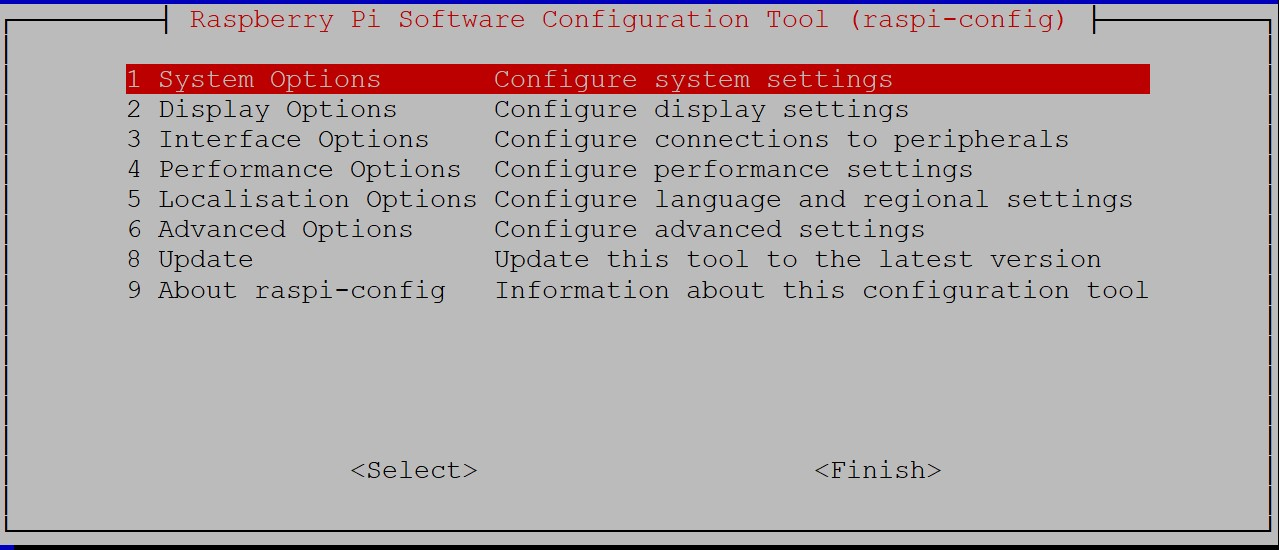
\includegraphics{./media/raspi-config.jpg}
\caption{raspi-config}
\end{figure}

\begin{verbatim}
    - change the default password of the user "pi":
        System Options/Password
    - enable the SSH, which has already been done for the Headless mode:
        Interface Options/SSH
    - reduce GPU memory to 16MB:
        Performance Options -> GPU memory
    - set locale settins:
        Localization Options
    - expand the filesystem to use the full capacity of the SD card:
        Advanced Options -> Expand Filesystem
    - disable [Predictable Network Interface Names](https://www.freedesktop.org/wiki/Software/systemd/PredictableNetworkInterfaceNames/):
        Advanced Options -> Network Interface Names
    - exit the *raspi-config* tool and reboot:
\end{verbatim}

\begin{Shaded}
\begin{Highlighting}[]
\ExtensionTok{$}\NormalTok{ sudo reboot now}
\end{Highlighting}
\end{Shaded}

\pagebreak

\begin{itemize}
\tightlist
\item
  Create the .ssh/authorized\_keys file on your RPi
\end{itemize}

\begin{Shaded}
\begin{Highlighting}[]
\CommentTok{\# Create the .ssh folder}
\BuiltInTok{cd}\NormalTok{ \textasciitilde{}}
\FunctionTok{mkdir}\NormalTok{ .ssh}
\CommentTok{\# Create the authorized\_keys file in the .ssh/}
\FunctionTok{touch}\NormalTok{ .ssh/authorized\_keys}

\CommentTok{\# Set proper access permissions}
\FunctionTok{chmod}\NormalTok{ 700 \textasciitilde{}/.ssh}
\FunctionTok{chmod}\NormalTok{ 600 \textasciitilde{}/.ssh/authorized\_keys}
\end{Highlighting}
\end{Shaded}

\begin{itemize}
\tightlist
\item
  Create the SSH key pair on your host machine
\end{itemize}

\begin{Shaded}
\begin{Highlighting}[]
\CommentTok{\# Check for existing key pair: id\_rsa and id\_rsa.pub}
\CommentTok{\# id\_rsa.pub\textquotesingle{}s content will be sent to other machines}
\CommentTok{\# !! id\_rsa is to be kept on your machine only}
\ExtensionTok{$}\NormalTok{ cd \textasciitilde{}/.ssh }\KeywordTok{\&\&} \FunctionTok{ls}

\CommentTok{\# Create the key pair, you can just save it in the default location \textasciitilde{}/.ssh/}
\ExtensionTok{$}\NormalTok{ cd \textasciitilde{}}
\ExtensionTok{$}\NormalTok{ ssh{-}keygen}

\CommentTok{\# Append the id\_rsa.pub to your RPi\textquotesingle{}s \textasciitilde{}/.ssh/authorized\_keys}
\ExtensionTok{$}\NormalTok{ ssh{-}copy{-}id pi@}\OperatorTok{\textless{}}\NormalTok{RPi\_private\_IP}\OperatorTok{\textgreater{}}
\CommentTok{\# Authenticate the process with your pi user\textquotesingle{}s password}
\end{Highlighting}
\end{Shaded}

\begin{itemize}
\item
  Installing Ansible

  \begin{itemize}
  \item
    What is Ansible? ``An Ansible playbook is a blueprint of automation
    tasks - which are complex IT actions executed with limited or no
    human involvement. Ansible playbooks are essentilaly frameworks,
    which are prewritten code that developers can use ad-hoc or as
    starting template.''
  \item
    It's possible to install Ansible directly on your RPi, but it isn't
    practical by doing so, since one of the benefits when using Ansible
    is the repeatability of it. For example if somehow your SD card gets
    ``bricked'' and you have to start over, this step and the one after
    can be re-ran right away.
  \item
    On a Linux machine, for example Ubuntu:
  \end{itemize}

\begin{Shaded}
\begin{Highlighting}[]
\CommentTok{\# Install pip3}
\ExtensionTok{$}\NormalTok{ sudo apt install python3{-}pip}
\CommentTok{\# Install Ansible version 5.2.0 (for reproducibility) with pip3}
\ExtensionTok{$}\NormalTok{ sudo pip3 install ansible==5.2.0}
\end{Highlighting}
\end{Shaded}

  \begin{itemize}
  \tightlist
  \item
    For Windows, Ansible isn't supported natively, so you must use WSL
    (\href{https://docs.microsoft.com/en-us/windows/wsl/install}{Windows
    Subsystem for Linux})
  \end{itemize}
\end{itemize}

\pagebreak

\begin{verbatim}
- Configuring "keep-alive" packets sending for SSH: to avoid the connection being closed due to inactivity and risk of disrupting Ansible
    Editing the */etc/ssh/ssh_config* file
\end{verbatim}

\begin{Shaded}
\begin{Highlighting}[]
\CommentTok{\# Look for the \textquotesingle{}Host *\textquotesingle{} line then add under it}
\ExtensionTok{ServerAliveInterval}\NormalTok{ 300}
\ExtensionTok{ServerAliveCountMax}\NormalTok{ 2}
\end{Highlighting}
\end{Shaded}

\begin{itemize}
\item
  Download and configure the Playbooks

  \begin{itemize}
  \tightlist
  \item
    Clone/Download from Andres's GitHub
  \end{itemize}

\begin{Shaded}
\begin{Highlighting}[]
\CommentTok{\# If you don\textquotesingle{}t have git installed}
\ExtensionTok{$}\NormalTok{ sudo apt install git}
\CommentTok{\# Clone the repo}
\ExtensionTok{$}\NormalTok{ git clone https://github.com/andresrcs/raspberry\_pi\_server.git }\AttributeTok{{-}{-}depth}\NormalTok{ 1}
\end{Highlighting}
\end{Shaded}

  \begin{itemize}
  \tightlist
  \item
    Define the ``inventory'' - the list of hosts to be connected to:
    edit the \emph{raspberry\_pi\_server/inventory.ini} file and add the
    IP of your RPi(s):
  \end{itemize}

\begin{Shaded}
\begin{Highlighting}[]
\CommentTok{\# This represents a group of Raspberries}
\ExtensionTok{[raspberries]}
\CommentTok{\# This is the hostname and IP for an individual Raspberry Pi}
\CommentTok{\# You can add as many Raspberries as you need}
\ExtensionTok{raspberry\_01}\NormalTok{ ansible\_host=192.168.0.10}
\end{Highlighting}
\end{Shaded}

  \begin{itemize}
  \tightlist
  \item
    Set common variables for your \texttt{{[}raspberries{]}} group: edit
    the \emph{rasberry\_pi\_server/group\_vars/raspberries.yml} file,
    pay attention to the path to the ssh key
  \end{itemize}

\begin{Shaded}
\begin{Highlighting}[]
\CommentTok{\# The default user for RPi is \textquotesingle{}pi\textquotesingle{}, change if needed}
\ExtensionTok{ansible\_user:}\NormalTok{ pi}
\ExtensionTok{ansible\_become\_method:}\NormalTok{ sudo}
\ExtensionTok{ansible\_python\_interpreter:}\NormalTok{ /usr/bin/python3}
\CommentTok{\# The location of the ssh key in your local host}
\ExtensionTok{ansible\_ssh\_private\_key\_file:}\NormalTok{ \textasciitilde{}/.ssh/raspberrypi\_key}
\end{Highlighting}
\end{Shaded}

  \begin{itemize}
  \tightlist
  \item
    Review the installation settings, the most important ones to look
    over are:
  \end{itemize}

\begin{Shaded}
\begin{Highlighting}[]
\CommentTok{\# Disable WiFi interface?}
\ExtensionTok{disable\_wifi:}\NormalTok{ false}

\CommentTok{\# Notification email for fail2ban}
\ExtensionTok{send\_email:}\NormalTok{ true}
\ExtensionTok{fail2ban\_email:}\NormalTok{ your\_email@something.com}

\CommentTok{\# Password for the main PostgreSQL user}
\ExtensionTok{postgres\_password:} \StringTok{\textquotesingle{}very\_secure\_password\textquotesingle{}}
\end{Highlighting}
\end{Shaded}
\end{itemize}

\pagebreak

\begin{itemize}
\item
  Run the Playbooks

  \begin{itemize}
  \tightlist
  \item
    the files to be executed are
  \end{itemize}

\begin{Shaded}
\begin{Highlighting}[]
\CommentTok{\# running everything at once}
\ExtensionTok{main.yml}

\CommentTok{\# runnig separately}
\ExtensionTok{install\_basic\_services.yml}
\ExtensionTok{install\_shiny\_server.yml}
\ExtensionTok{install\_rstudio\_server.yml}
\end{Highlighting}
\end{Shaded}

  \begin{figure}
  \centering
  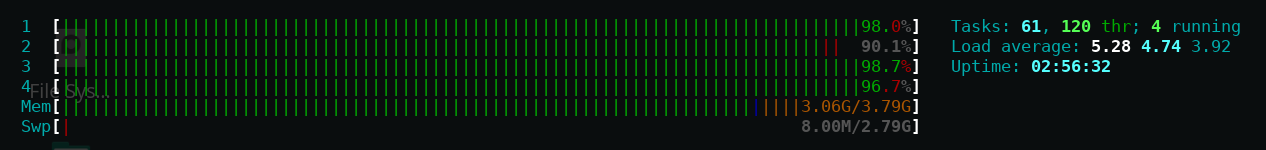
\includegraphics{./media/2_pushedToLimit.png}
  \caption{Pushed to the limit}
  \end{figure}

  \begin{itemize}
  \tightlist
  \item
    It is recommended to run them separately, since the whole
    installation process can take up to 6 hours, and will be easier for
    troubleshooting. The command to used is
  \end{itemize}

\begin{Shaded}
\begin{Highlighting}[]
\ExtensionTok{$}\NormalTok{ ansible{-}playbook }\OperatorTok{\textless{}}\NormalTok{playbook}\OperatorTok{\textgreater{}}
\end{Highlighting}
\end{Shaded}

  \begin{itemize}
  \tightlist
  \item
    For a more specific use cases of the playbooks, there are
    \href{https://andresrcs.rbind.io/2021/01/13/raspberry_pi_server/\#run-the-playbooks}{``tags''}
    to run only part of the playbooks, such as
  \end{itemize}

\begin{Shaded}
\begin{Highlighting}[]
\CommentTok{\# \textquotesingle{}r\textquotesingle{} for the actual tag\textquotesingle{}s name}
\ExtensionTok{$}\NormalTok{ ansible{-}playbook install\_basic\_services.yml }\AttributeTok{{-}{-}tags} \StringTok{"r"}
\end{Highlighting}
\end{Shaded}
\item
  After the playbooks finish running, you should now have a functional
  RStudio + Shiny Server on your RPi, access them through:

  \begin{itemize}
  \tightlist
  \item
    http://RPi\_private\_IP/rstudio for RStudio session, or enter in the
    terminal the command: \texttt{\$\ R}
  \item
    http://RPi\_private\_IP/shiny/app\_name to access your shiny apps,
    source code files are to be kept in
    \emph{/srv/shiny-server/app\_name/} folder.
  \end{itemize}
\end{itemize}

\newpage

\hypertarget{pmm}{%
\subsection{PMM}\label{pmm}}

\hypertarget{brief-introduction-1}{%
\subsubsection{Brief introduction}\label{brief-introduction-1}}

\hypertarget{development}{%
\subsubsection{Development}\label{development}}

\hypertarget{security-measures}{%
\subsubsection{Security measures}\label{security-measures}}

\hypertarget{deployment}{%
\subsubsection{Deployment}\label{deployment}}

\hypertarget{port-forwarding}{%
\paragraph{Port Forwarding}\label{port-forwarding}}

This function is varied from manufactures to manufactures and also
depending on their models, but the overall settings won't be too much of
a difference from the following:

\begin{figure}
\centering
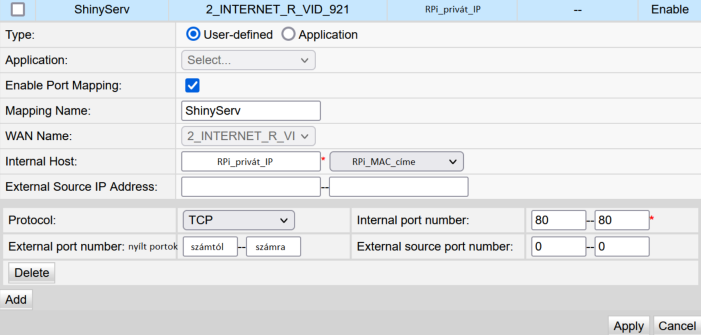
\includegraphics{./media/portForwarding.png}
\caption{A Huawei router's Port Forwarding}
\end{figure}

\hypertarget{ddns-service---noip}{%
\paragraph{DDNS service - NoIP}\label{ddns-service---noip}}

\newpage

\hypertarget{possible-problems-and-their-solutions}{%
\section{Possible problems and their
solutions}\label{possible-problems-and-their-solutions}}

\newpage

\hypertarget{results}{%
\section{Results}\label{results}}

\newpage

\hypertarget{dicussion}{%
\section{Dicussion}\label{dicussion}}

\newpage

\hypertarget{conclusion}{%
\section{Conclusion}\label{conclusion}}
